\documentclass[class=article,border=5pt,tikz]{standalone}
\usetikzlibrary{calc,intersections,through,backgrounds}
\usetikzlibrary{spy}

\tikzset{fig/.pic={code={%

      % coordinates to be reused
      \coordinate (A) at (0,0);
      \coordinate (B) at (1,0);
      \coordinate (C) at (1,1);
      \coordinate (D) at (0,1);
      \coordinate (P) at (0,0.16667);
      \coordinate (Q) at (1,0.16667);
      \path [name path=DB] (D) -- (B);
      \path [name path=CP] (C) -- (P);
      \path [name path=DQ] (D) -- (Q);
      \path [name path=CA] (C) -- (A);
      \path [name intersections={of=CA and DB, by=a}];
      \path [name intersections={of=DB and CP, by=b}];
      \path [name intersections={of=DQ and CP, by=c}];
      \path [name intersections={of=CA and DQ, by=d}];
      
      % draw figure
      \begin{scope}
      \draw (A) -- (B) -- (C) -- (D) -- cycle;
      \draw (C) -- (P);
      \draw (D) -- (Q);
      \draw (C) -- (A);
      \draw (D) -- (B);
      \end{scope}
                  
      % add labels
      \node [below left] at (A) {A};
      \node [below right] at (B) {B};
      \node [above right] at (C) {C};
      \node [above left] at (D) {D};
      \node [left] at (P) {P};
      \node [right] at (Q) {Q};
      
}}}%

\begin{document}
% main figure
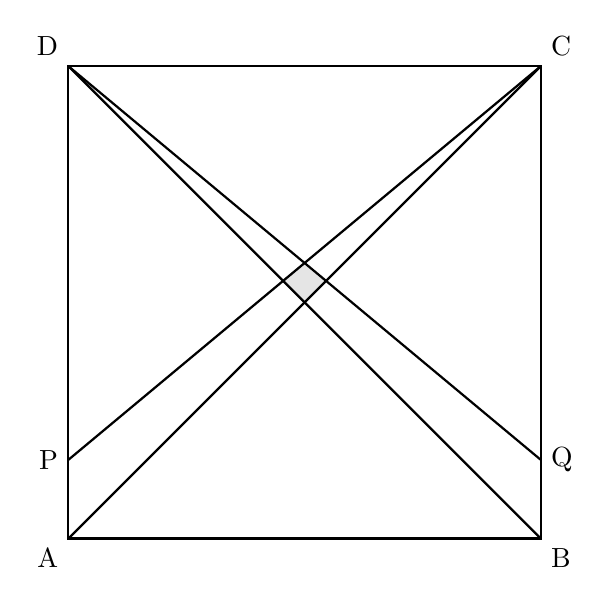
\begin{tikzpicture}[thick, x=6cm, y=6cm]
    \path (0,0) pic {fig};
    \begin{pgfonlayer}{background}% background otherwise it 'leaks'
      \draw [fill=gray!20] (a) -- (b) -- (c) -- (d);
    \end{pgfonlayer}
\end{tikzpicture}

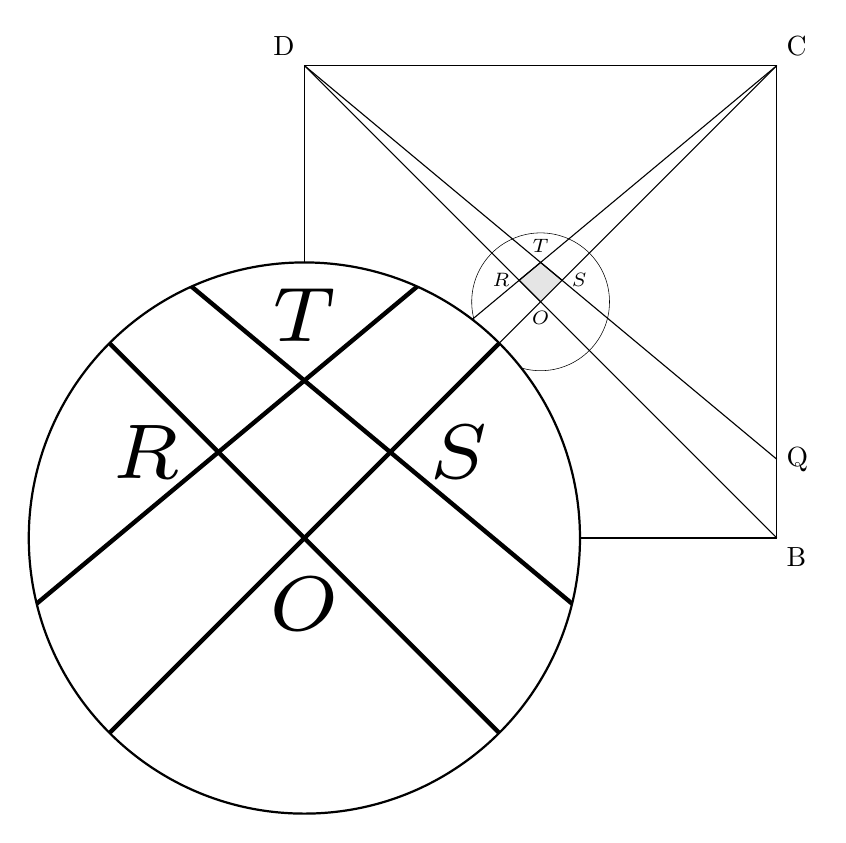
\begin{tikzpicture}[thick, x=6cm, y=6cm, spy using outlines={circle, magnification=4, size=7cm, connect spies}]
    \path (1.5,0) pic {fig};
    \begin{pgfonlayer}{background}% background otherwise it 'leaks'
      \draw [fill=gray!20] (a) -- (b) -- (c) -- (d);
    \end{pgfonlayer}
    % add labels
    \node [below,font=\scriptsize] at (a) {$O$};
    \node [left, font=\scriptsize] at (b) {$R$};
    \node [above,font=\scriptsize] at (c) {$T$};
    \node [right,font=\scriptsize] at (d) {$S$};
    \spy on (a) in node [fill=white] at (A);
\end{tikzpicture}

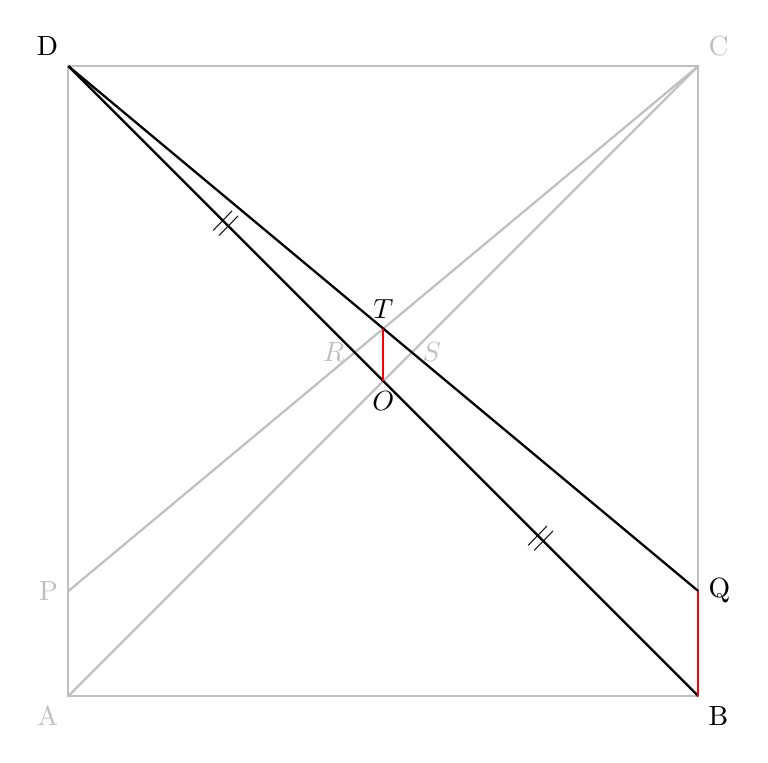
\begin{tikzpicture}[thick, x=8cm, y=8cm]
    \path (0,0) pic[lightgray] {fig};
    \draw (D) -- (B);
    \draw (D) -- (Q);
    \draw [red] (B) -- (Q);
    \draw [red] (a) -- (c);
    \node [above left] at (D) {D};
    \node [below right] at (B) {B};
    \node [right] at (Q) {Q};
    \node [below] at (a) {$O$};
    \node [left,lightgray] at (b) {$R$};
    \node [above] at (c) {$T$};
    \node [right,lightgray] at (d) {$S$};
    \path (a) -- (B) node [midway,rotate=-44] {$||$};
    \path (D) -- (a) node [midway,rotate=-44] {$||$};
\end{tikzpicture}


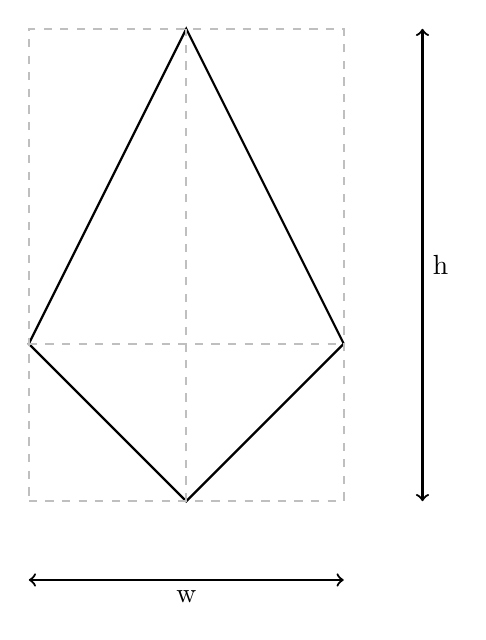
\begin{tikzpicture}[thick,scale=2]
    \draw (0,0) -- (1,1) -- (0,3) -- (-1,1) -- cycle;
    \draw [dashed,lightgray] (0,0) -- (0,3);
    \draw [dashed,lightgray] (-1,1) -- (1,1);
    \draw [<->] (1.5,0) -- (1.5,3) node [midway,right] {h};
    \draw [<->] (-1,-0.5) -- (1,-0.5) node [midway,below] {w};
    \draw [dashed,lightgray] (-1,0) -- (1,0) -- (1,3) -- (-1,3) -- cycle;
\end{tikzpicture}



\begin{tikzpicture}[thick,x=2cm, y=2cm]
    % set coordinates
    \coordinate (A) at (0,0);
    \coordinate (M) at (5,2);
    \coordinate (N) at (5,-2);
    \coordinate (P) at (0,-1.8);
    \coordinate (Q) at (2,2.5);
    \coordinate (R) at (2,-1.8);
    \coordinate (S) at (4,2.5);
    % define paths
    \path [name path=AM] (A) -- (M);
    \path [name path=AN] (A) -- (N);
    \path [name path=PQ] (P) -- (Q);
    \path [name path=RS] (R) -- (S);
    % define intersections
    \path [name intersections={of=AM and PQ, by=B}];
    \path [name intersections={of=AM and RS, by=C}];
    \path [name intersections={of=AN and PQ, by=D}];
    \path [name intersections={of=AN and RS, by=E}];
    % draw figure
    \draw (A) -- (M);
    \draw (A) -- (N);
    \draw (P) -- (Q);
    \draw (R) -- (S);
    % add labels
    \node [left] at (A) {A};
    \node [above left] at (B) {B};
    \node [above left] at (C) {C};
    \node [below left,shift={(-5pt,-1pt)}] at (D) {D};
    \node [below left,shift={(-5pt,-1pt)}] at (E) {E};
\end{tikzpicture}



\begin{tikzpicture}
\node[font=\huge]{TO DO};
\end{tikzpicture}

\end{document}
